\documentclass{article}

\author{Teddy Krulewich}
\title{\vspace{-4em}HW4 ME5501 – Robotics and Unmanned Systems}

\usepackage{graphicx}
\graphicspath{ {images/} }


\usepackage[utf8]{inputenc}
\usepackage{minted}
\usepackage{hyperref}
\usepackage{xcolor}
\definecolor{bg}{rgb}{0.95,0.95,0.95}
\usepackage{caption}
\usepackage{mdframed}

\begin{document}
\maketitle

\section*{Problem 1}
Complete the following ROS tutorials at \url{https://docs.ros.org/en/foxy/Tutorials.html}

• Understanding ROS Nodes

• Understanding ROS Topics

\bigskip
\noindent Save a screenshot of the Turtlebot simulator and show/print the screenshot.


\begin{figure}[H]
    \centering
    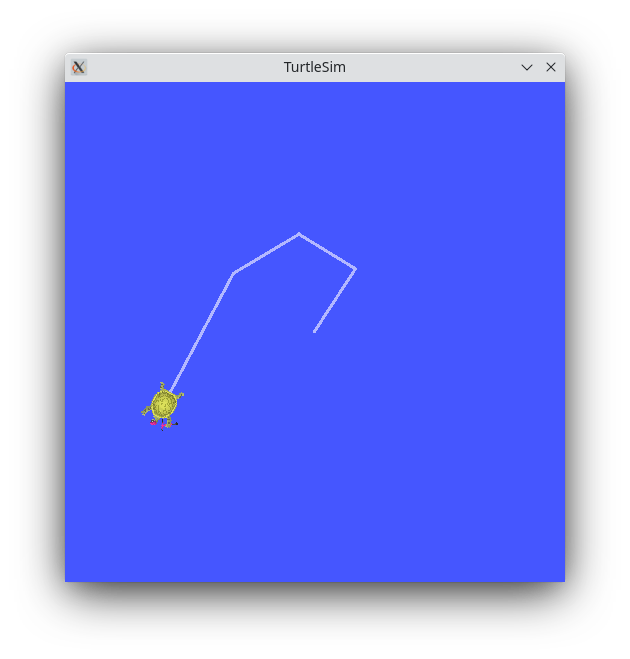
\includegraphics[width=0.5\textwidth]{question1.png}
    \caption*{Screenshot of Turtlebot Simulator}
\end{figure}

\section*{Problem 2}

Complete the following ROS tutorials at

\url{http://wiki.ros.org/ROS/Tutorials}


• 12. Writing a Simple Publisher and Subscriber (Python) 


• 13. Examining the Simple Publisher and Subscriber 

\bigskip 
\noindent Save a screenshot of the running code in tutorials 13, and print these screenshots to turn in.

\begin{figure}[H]
    \centering
    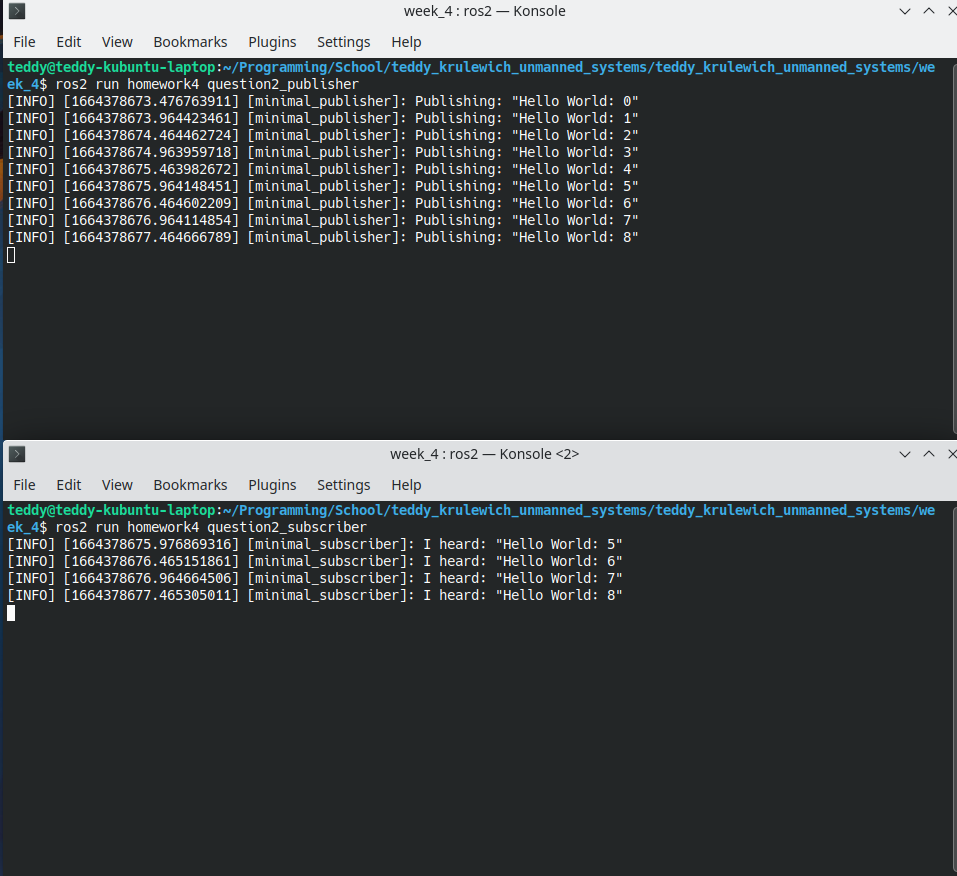
\includegraphics[width=\textwidth]{question2.png}
    \caption*{Screenshot of subscriber and publisher running}
\end{figure}

\bigskip
\section*{Problem 3}

For this problem you will be using ROS2 and Gazebo to simulate the Turtlebot3 Burger platform.  
Help in loading the simulation can be found at 
\url{http://emanual.robotis.com/docs/en/platform/turtlebot3/simulation/}.

\bigskip
\noindent Make sure to go to the Gazebo part of the E-manual. When setting the model type, replace “\$\{TB3\_MODEL\}” with 
“burger.” 

\bigskip
\noindent Create a ROS2 node that makes the Turtlebot3 travel forward at 1.5 m/s (remember this speed is 
much faster than it can do in real life) for 5 seconds, then turns to the right at 0.15 rad/s for 2 
seconds, then continues forward at 1.5 m/s for another 5 seconds before stopping. Log the position 
data, and velocity \& angular velocity commands.

\bigskip 
\noindent Create a subplot of the x \& y position data, velocity \& angular velocity commands versus time. 

\bigskip
\noindent Submit your Python code.

\begin{figure}[H]
    \centering
    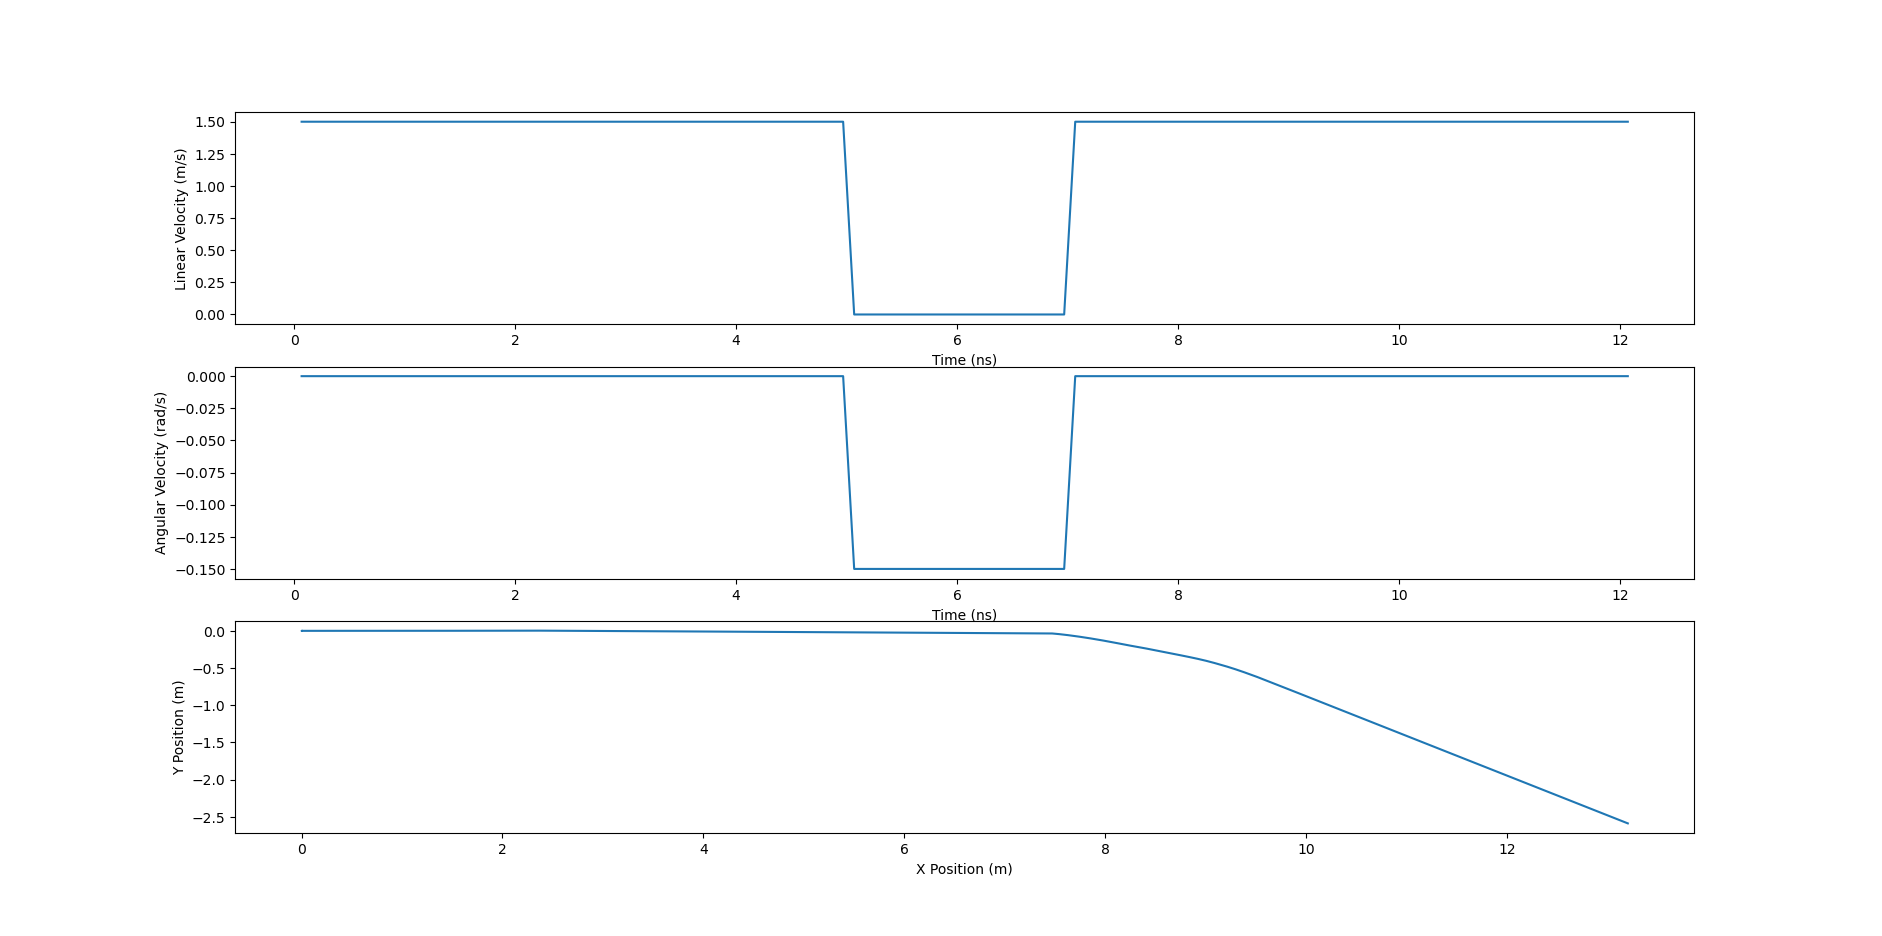
\includegraphics[width=\textwidth]{question3.png}
    \caption*{Plot of position data, velocity, and angular velocity commands versus time}
\end{figure}

\begin{minted}[bgcolor=bg,fontsize=\footnotesize,linenos]{python}
\end{minted}

\section*{Problem 4}
Create a ROS2 node/script that uses a feedback controller to control the heading of the Turtlebot3. 
Once you have adequately tuned the controller, collect the data (by writing to a log file) from a 90 
degree step input (use a forward speed of 0.15 m/s).

\bigskip
\noindent Create a plot of the desired and actual heading versus time. What is the rise time, settling time, and 
percent overshoot of your controller? 

\bigskip
\noindent Submit your Python code.

\begin{figure}[H]
    \centering
    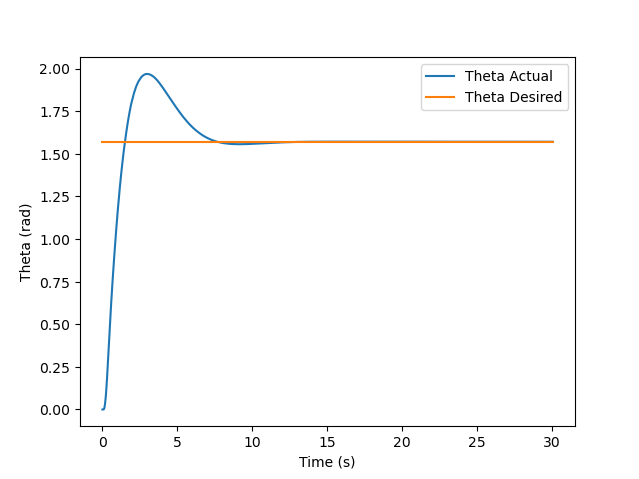
\includegraphics[width=\textwidth]{question4.png}
    \caption*{Plot of desired and actual heading versus time}
\end{figure}

\end{document}